\documentclass[11pt]{amsart}
%\pagestyle{empty} 
\setlength{\topmargin}{-0.75in} % usually -0.25in
\addtolength{\textheight}{1.25in} % usually 1.25in
\addtolength{\oddsidemargin}{-1.2in}
\addtolength{\evensidemargin}{-1.2in}
\addtolength{\textwidth}{1.9in} %\setlength{\parindent}{0pt}

\newcommand{\normalspacing}{\renewcommand{\baselinestretch}{1.1}\tiny\normalsize}
\normalspacing

% macros
\usepackage{amssymb,xspace,alltt,verbatim}
\usepackage[final]{graphicx}
\usepackage[pdftex,colorlinks=true]{hyperref}
\usepackage{fancyvrb}
\usepackage{tikz}

\newtheorem*{lem*}{Lemma}

\newcommand{\bb}{\mathbf{b}}
\newcommand{\bc}{\mathbf{c}}
\newcommand{\bs}{\mathbf{s}}
\newcommand{\bu}{\mathbf{u}}
\newcommand{\bv}{\mathbf{v}}
\newcommand{\bw}{\mathbf{w}}
\newcommand{\bx}{\mathbf{x}}
\newcommand{\by}{\mathbf{y}}

\newcommand{\bbf}{\mathbf{f}}

\newcommand{\CC}{{\mathbb{C}}}
\newcommand{\RR}{{\mathbb{R}}}
\newcommand{\eps}{\epsilon}
\newcommand{\ZZ}{{\mathbb{Z}}}
\newcommand{\ZZn}{{\mathbb{Z}}_n}
\newcommand{\NN}{{\mathbb{N}}}
\newcommand{\ip}[2]{\mathrm{\left<#1,#2\right>}}

\renewcommand{\Re}{\operatorname{Re}}
\renewcommand{\Im}{\operatorname{Im}}

\newcommand{\Log}{\operatorname{Log}}

\newcommand{\grad}{\nabla}

\newcommand{\ds}{\displaystyle}

\newcommand{\Matlab}{\textsc{Matlab}\xspace}
\newcommand{\Octave}{\textsc{Octave}\xspace}
\newcommand{\pylab}{\textsc{pylab}\xspace}

\newcommand{\prob}[1]{\bigskip\noindent\textbf{#1.} }
\newcommand{\cprob}[1]{\bigskip\noindent\underline{\textbf{#1.}} }
\newcommand{\pts}[1]{(\emph{#1 pts})}

\newcommand{\probpts}[2]{\prob{#1} \pts{#2} \quad}
\newcommand{\cprobpts}[2]{\cprob{#1} \pts{#2} \quad}
\newcommand{\ppartpts}[2]{\textbf{(#1)} \pts{#2} \quad}
\newcommand{\epartpts}[2]{\medskip\noindent \textbf{(#1)} \pts{#2} \quad}


\begin{document}
\hfill \Large Name:\underline{\phantom{Ed Bueler really really long long long name}}
\medskip

\scriptsize \noindent Math 252 Calculus 2 (Bueler) \hfill Wednesday, 27 April 2022
\medskip

\LARGE\centerline{\textbf{Final Exam}}

\smallskip
\begin{quote}
\large
\textbf{No book, electronics, calculator, or internet access.  125 points possible.  125 minutes maximum.}

\textbf{Allowed notes: 1/2 sheet of letter paper (i.e.~$8.5\times 11$ paper) allowed, with anything written on both sides.}
\end{quote}

\normalsize
\medskip

\thispagestyle{empty}

\cprob{1}  Evaluate the definite and indefinite integrals:

\epartpts{a}{6} $\ds  \int_0^{\pi/2} \sin^3 \theta\,d\theta =$
\vspace{2.5in}

\epartpts{b}{6} $\ds  \int \sqrt{25 - x^2}\,dx =$
\vfill


\clearpage\newpage
\prob{2}  Evaluate the indefinite integrals:

\epartpts{a}{6} $\ds  \int t\, 3^{t}\,dt =$
\vfill

\epartpts{b}{6} $\ds  \int \frac{dx}{(x+1)(x-3)} =$
\vfill


\clearpage\newpage
\cprob{3}  \ppartpts{a}{5} Sketch the region bounded by $\displaystyle y=\frac{1}{4} x^2$, the $y$-axis, and the line $y=1$.
\vfill

\epartpts{b}{8} Compute the volume of the solid of revolution found by rotating the region in \textbf{(a)} around the $x$-axis.  Simplify your answer.
\vfill


\clearpage\newpage
\cprobpts{4}{8}  Compute the improper integral.  Use appropriate limit notation.
    $$\int_1^\infty x e^{-x^2/2}\,dx = \hspace{5.0in}$$
\vfill

\cprob{5}  Determine whether the following series converge or diverge. Explain your reasoning and identify any test used.

\epartpts{a}{6}  $\ds \sum_{n = 1}^\infty \frac{\sqrt{n}}{12 + n}$
\vfill

\epartpts{b}{6}  $\ds \sum_{n = 2}^\infty (-1)^n\frac{\ln n}{n}$
\vspace{1.5in}


\clearpage\newpage
\cprobpts{6}{8}  Find the radius and interval of convergence of the power series:
    $$\sum_{n = 1}^\infty \frac{(-1)^n(x + 2)^n}{3^n\sqrt n} \hspace{5.0in}$$
\vfill

\cprobpts{7}{8}  Find the Taylor series for the function $f(x) = e^{2x}$ centered at the point $a = -3$. Give your answer in summation notation.
\vspace{3.0in}


\clearpage\newpage
\cprobpts{8}{8}  Find the arc length of the parametric curve defined by $\displaystyle x = 1 - \frac13t^3$, $y = t^2 + 3$ on the interval $0\leq t\le 4$.
\vfill

\probpts{9}{6}  How accurate is the approximation of $\ds \sum_{n=1}^\infty \frac{(-1)^{n+1}}{n}$ by its partial sum $S_{100}$?  Write a correct bound in the box and give a brief justification.

   $$\left|\sum_{n=1}^\infty \frac{(-1)^{n+1}}{n} - S_{100}\right| \le \boxed{\phantom{\begin{matrix} lakjsd alsfjd sadf \\ sdfa \\ sdaf \end{matrix}}} \hspace{4.0in}$$
\vspace{2.0in}


\clearpage\newpage
\prob{10} \ppartpts{a}{5}  Does the series $\ds \sum_{n=1}^\infty \frac{n}{2^n}$ converge or diverge?  Explain your reasoning and identify any test used.
\vspace{3.0in}

\epartpts{b}{8}  Evaluate (find the sum for) the series in \textbf{(a)} by computing $\ds f'\left(\frac{1}{2}\right)$ where
  $$f(x) = \sum_{n=0}^\infty x^n = \frac{1}{1-x}. \hspace{5.0in}$$
\vfill


\clearpage\newpage
\prob{11}  Consider the parametric curve $x = t + \cos t$, $y = t - \sin t$.

\epartpts{a}{6}  Find the equation of the tangent line at $t=\pi$.
\vfill

\epartpts{b}{6}  Compute the second derivative $\ds \frac{d^2 y}{dx^2}$.
\vfill


\clearpage\newpage
\prob{12} \ppartpts{a}{5}  Make a careful and reasonably-large sketch of the cardiod $r = 1 + \sin\theta$.  (\emph{Label the axes and give dimensions/values along the axes.})
\vfill

\epartpts{b}{8}  Find the area inside the cardioid in \textbf{(a)}.
\vfill


\clearpage\newpage
\probpts{Extra Credit}{3}  These two polar curves both spiral toward the origin:

\medskip
\textbf{A.\,} $\ds \strut r=e^{-\theta}$ on $0\le \theta < \infty$

\medskip
\textbf{B.\,} $\ds r = \frac{1}{\strut\theta}$ on $1\le \theta < \infty$

\noindent However, one has finite arclength and the other infinite.  Which is which?  Find the length of the finite one \emph{and} show the other has infinite length.
\vfill

\noindent \hrule
\begin{center}
\small
\bigskip
\textsc{blank space}
\end{center}
\vspace{3.0in}


\clearpage\newpage
\large\centerline{\textbf{Summary of Convergence Tests}}
\normalsize

\begin{center}
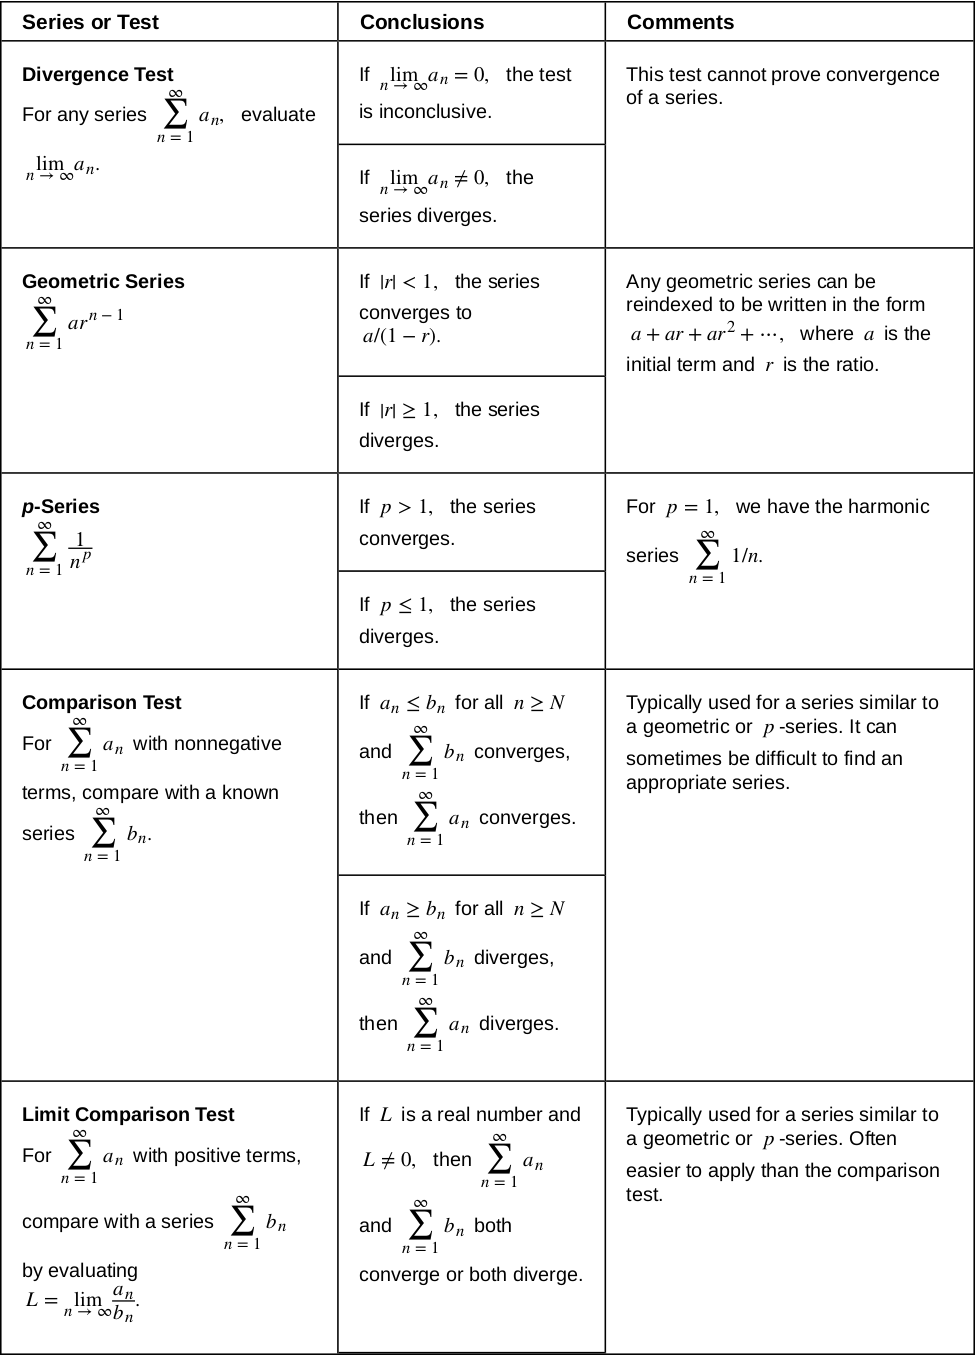
\includegraphics[width=0.95\textwidth]{figs/serieshandoutA.png}
\end{center}
\vfill


\clearpage\newpage
\begin{center}
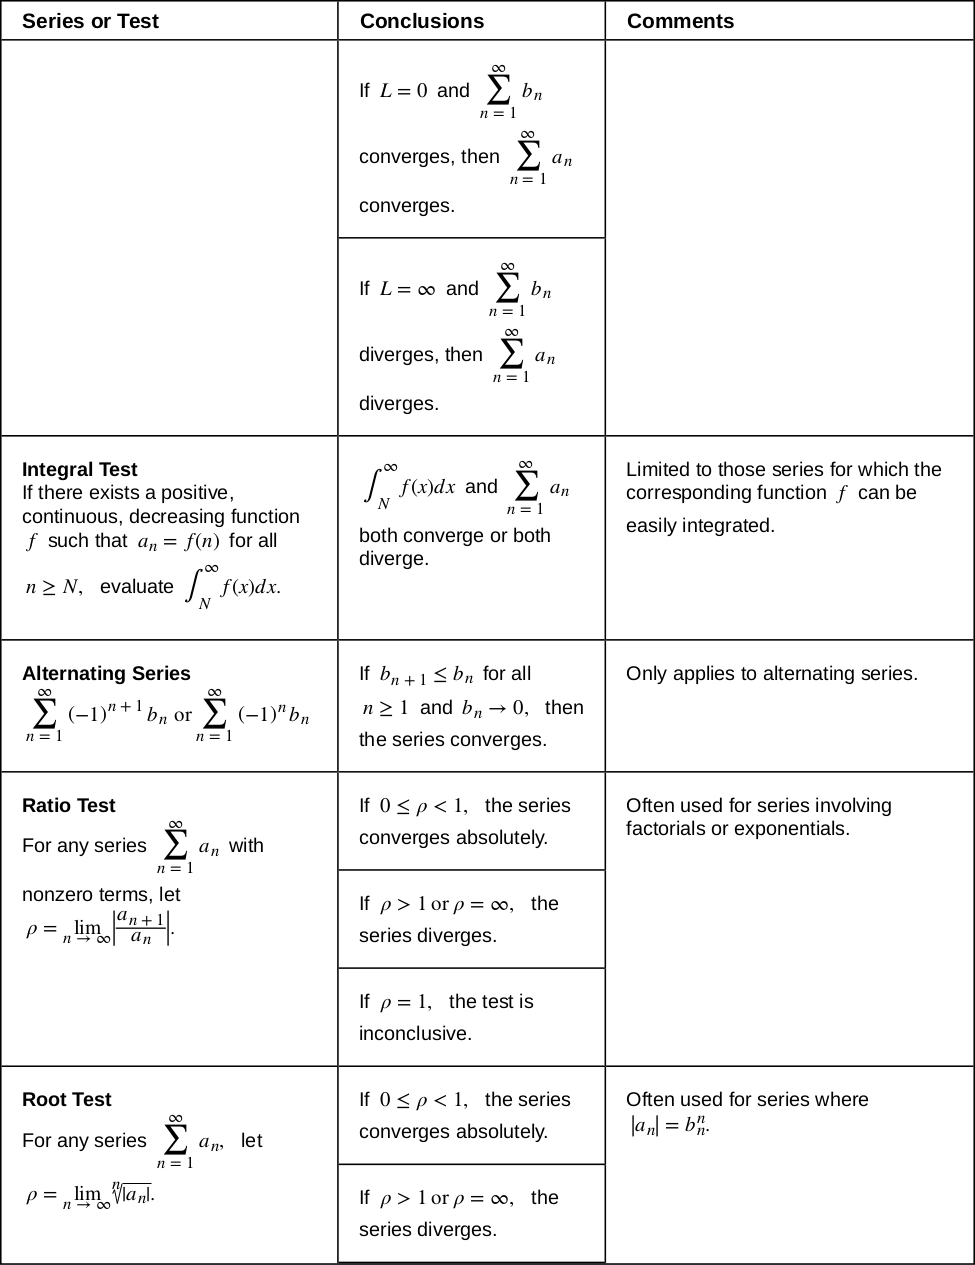
\includegraphics[width=0.95\textwidth]{figs/serieshandoutB.png}

\vspace{-2mm}
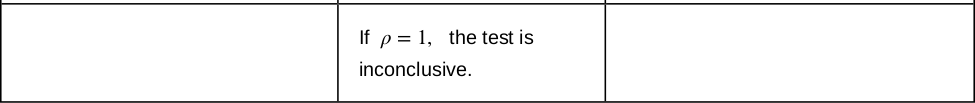
\includegraphics[width=0.95\textwidth]{figs/serieshandoutC.png}
\end{center}
\vfill

\end{document}
